\documentclass[10pt, aspectratio=169]{beamer}

\usepackage{svg}
\usepackage[absolute,overlay]{textpos}
\usepackage{fontspec}
\usetheme[progressbar=foot]{metropolis}
\setbeamercolor{background canvas}{bg=white}

\setbeamertemplate{section page}{
    \begin{minipage}{\textwidth}
        \centering
        \usebeamercolor[fg]{section title}
        \usebeamerfont{section title}
        \textsc{\insertsection}\par
        \vspace{1cm}
    \end{minipage}
    \begin{minipage}{\textwidth}
        \usebeamercolor[fg]{normal text}
        \tiny\tableofcontents[currentsection]
    \end{minipage}
}

\usepackage{hyperref}
\hypersetup{
    colorlinks = true,
    urlcolor = blue,
    linkcolor = black
}

\usepackage[scale=1]{ccicons}

% Code listings
\usepackage{minted}
\usepackage{caption}
\usepackage{xcolor}
% New command that includes caption with the file path
\captionsetup[listing]{labelformat=empty}
\newcommand{\inputmintedpath}[2]{
  \begin{listing}[H]
    \inputminted[
      linenos,
      numbersep=15pt,
      framesep=2mm,
      bgcolor=lightgray!20,
      baselinestretch=1.1,
      fontsize=\scriptsize,
      firstnumber=1,
      stepnumber=5,
    ]{#1}{#2}
    \caption{\scriptsize\texttt{\detokenize{#2}}} % Caption (file path)
  \end{listing}
}

\setbeameroption{hide notes} % Only slides
%\setbeameroption{show only notes} % Only notes
%\setbeameroption{show notes on second screen=right} % Both
% Add notes like this: \note{Note}

% Make surethat parskip is properly adjusted also in columns
\renewcommand{\baselinestretch}{1.3}
\makeatletter
\newcommand{\@minipagerestore}{\setlength{\parskip}{0.65em}}
\makeatother

\metroset{titleformat frame=smallcaps}
\newcommand{\parspace}{\vspace{1em}}


\title{Hands-on Zephyr Project Workshop}
\subtitle{Navigating Low Power IoT Development with Practical Examples}
\author{Jonas Remmert}
\institute{IoT Embedded Systems Engineer at Phytec Messtechnik GmbH}
\date{\today}

\begin{document}
%%%%%%%%%%%%%%%%%%%%%%%%%%%%%%%%%%%%%%%%%%%%%%%%%%%%%%%%%%%%%%%%%%%%%%%%%%%%%%%
\begin{frame}
    \vspace*{0.5cm}  % Adjust the length here for moving the title down.
    \titlepage
\end{frame}
%%%%%%%%%%%%%%%%%%%%%%%%%%%%%%%%%%%%%%%%%%%%%%%%%%%%%%%%%%%%%%%%%%%%%%%%%%%%%%%
\begin{frame}{Table of contents}
  \setbeamertemplate{section in toc}[sections numbered]
  \tableofcontents[]
\end{frame}
%%%%%%%%%%%%%%%%%%%%%%%%%%%%%%%%%%%%%%%%%%%%%%%%%%%%%%%%%%%%%%%%%%%%%%%%%%%%%%%
\section{Introduction}
% Introduce myself
% Set the stage for the workshop
% Explain the goals of the workshop
% Introduction to Zephyr
%%%%%%%%%%%%%%%%%%%%%%%%%%%%%%%%%%%%%%%%%%%%%%%%%%%%%%%%%%%%%%%%%%%%%%%%%%%%%%%
\begin{frame}[fragile]{Welcome and Professional Background}
  \begin{columns}
    \begin{column}{0.6\textwidth}
      \begin{description}
        \item Jonas Remmert
        \item Phytec Messtechnik GmbH
        \item Developer for Low Power IoT products
        \item[Experience] RTOS (FreeRTOS, Zephyr), NXP MCUX, hardware development
        \item[Focus Area] Firmware and hardware development with Nordic nRF9160 SoC
      \end{description}
    \end{column}
    \begin{column}{0.4\textwidth}
    \end{column}
  \end{columns}
\end{frame}
%%%%%%%%%%%%%%%%%%%%%%%%%%%%%%%%%%%%%%%%%%%%%%%%%%%%%%%%%%%%%%%%%%%%%%%%%%%%%%%
\begin{frame}[fragile]{Areas of Work and Contributions}
  \begin{columns}
    \begin{column}{0.5\textwidth}
      \begin{description}
        \item[Zephyr:] Contributor to Zephyr Project
        \item[Hardware:] Customer-specific hardware solutions, focus on low-power embedded systems
        \item[nRF9160 SoC:] Developmment of IoT applications using the Nordic nRF9160 SoC for both hardware and firmware
      \end{description}
    \end{column}
    \begin{column}{0.4\textwidth}
      \begin{figure}
        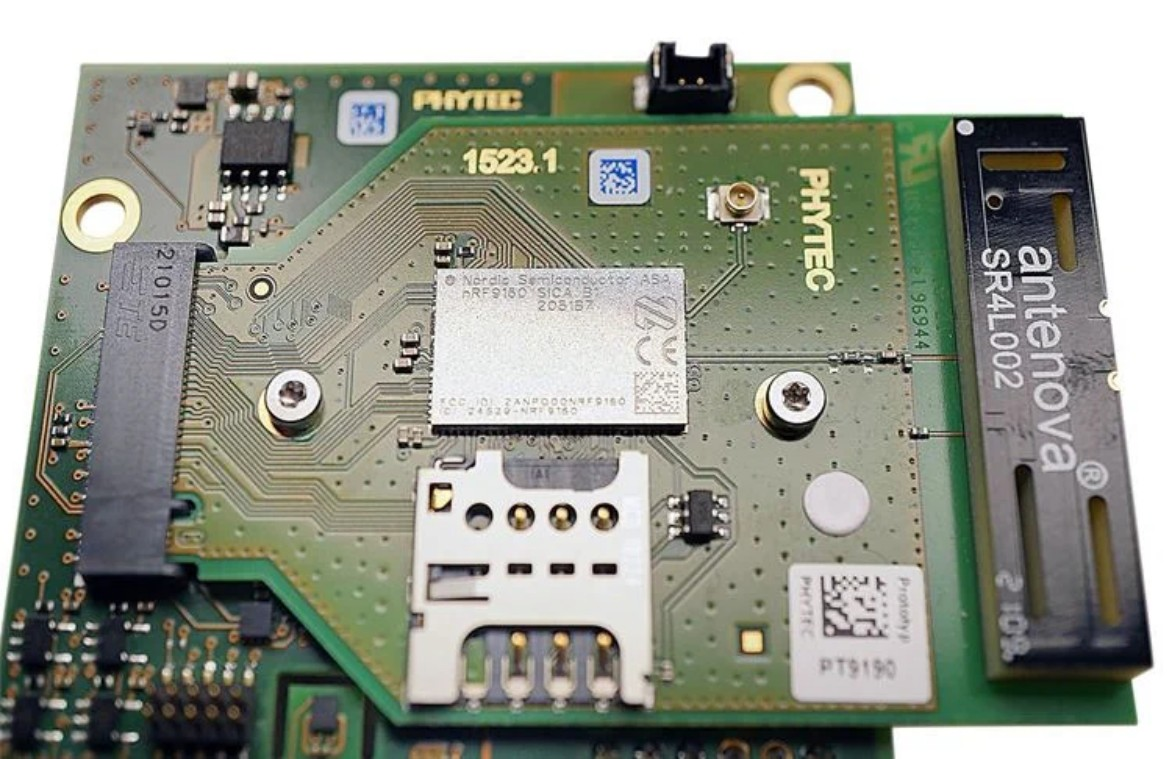
\includegraphics[width=0.8\textwidth]{images/jrov2201.jpg}
        \caption{Pump Monitor, developed in collaboration with BeST Berliner Sensortechnik GmbH}
      \end{figure}
    \end{column}
  \end{columns}
\end{frame}
%%%%%%%%%%%%%%%%%%%%%%%%%%%%%%%%%%%%%%%%%%%%%%%%%%%%%%%%%%%%%%%%%%%%%%%%%%%%%%%
\begin{frame}[fragile]{Workshop Goals}
  \begin{columns}[]
    \begin{column}{0.6\textwidth}
      \begin{itemize}
        \item Merge theory with hands-on practice
        \item Introduction to Zephyr RTOS
        \item Zephyr setup guide
          \begin{itemize}
            \item Local setup
            \item GitHub Codespaces configuration
          \end{itemize}
        \item Exploring some of Zephyr's key features
        \item Hands-on Sessions
          \begin{enumerate}
            \item Development environment setup
            \item Build and test samples
            \item Build Zephyr for different boards
            \item Extend an application
          \end{enumerate}
      \end{itemize}
    \end{column}
    \begin{column}{0.4\textwidth}
    \end{column}
  \end{columns}
\end{frame}
%%%%%%%%%%%%%%%%%%%%%%%%%%%%%%%%%%%%%%%%%%%%%%%%%%%%%%%%%%%%%%%%%%%%%%%%%%%%%%%
\begin{frame}[fragile]{Workshop Goals - Audience}
  \begin{columns}[]
    \begin{column}{0.6\textwidth}
      \begin{itemize}
        \item What are your goals for the Workshop?
        \item Have you used an RTOS before?
        \item Your experience with Zephyr?
      \end{itemize}
    \end{column}
    \begin{column}{0.4\textwidth}
    \end{column}
  \end{columns}
\end{frame}
%%%%%%%%%%%%%%%%%%%%%%%%%%%%%%%%%%%%%%%%%%%%%%%%%%%%%%%%%%%%%%%%%%%%%%%%%%%%%%%
\begin{frame}[fragile]{Introduction to the Zephyr Project}
  \begin{columns}
    \begin{column}{0.6\textwidth}
      \begin{itemize}
        \item More than an RTOS, IoT ecosystm
        \item Microcontrollers, wireless SoCs to multicore SoCs
        \item Alternative to vendor-specific SDKs
        \item Industry increasingly adopts Zephyr
        \item Set to be primary IoT ecosystem, if resource constraints do not allow to run Linux
      \end{itemize}
    \end{column}
    \begin{column}{0.4\textwidth}
      \begin{figure}
        
\includegraphics[width=0.8\textwidth]{images/zephyr_logo.png}
        \caption*{The Zephyr Project logo}
      \end{figure}
    \end{column}
  \end{columns}
\end{frame}
%%%%%%%%%%%%%%%%%%%%%%%%%%%%%%%%%%%%%%%%%%%%%%%%%%%%%%%%%%%%%%%%%%%%%%%%%%%%%%%
\begin{frame}[fragile]{Introduction to the Zephyr Project}
  \begin{figure}
    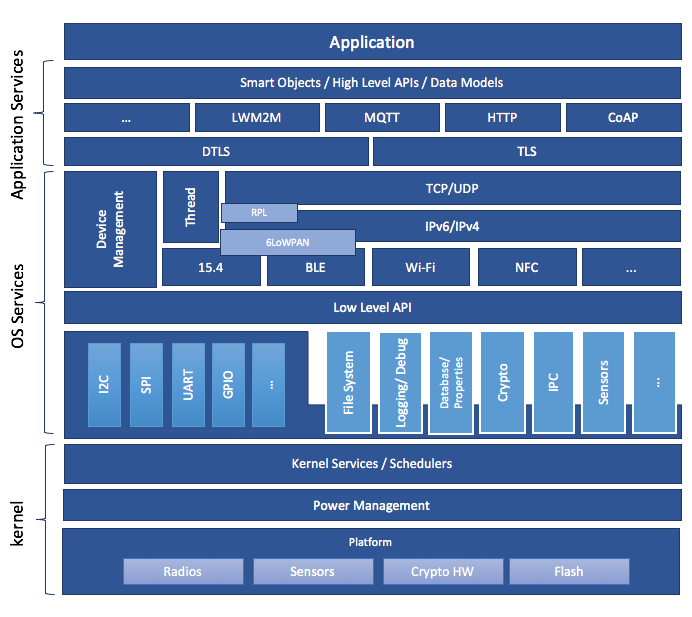
\includegraphics[width=0.55\textwidth]{images/system-architecture.png}
    \caption*{\href{https://docs.zephyrproject.org/latest/security/security-overview.html}{docs.zephyrproject.org/latest/security/security-overview.html}}
  \end{figure}
\end{frame}
%%%%%%%%%%%%%%%%%%%%%%%%%%%%%%%%%%%%%%%%%%%%%%%%%%%%%%%%%%%%%%%%%%%%%%%%%%%%%%%
\begin{frame}[fragile]{Open Source and Vendor-Neutral Governance}
  \begin{columns}
    \begin{column}{0.6\textwidth}
      \begin{itemize}
        \item Managed by Linux Foundation.
        \item Vendor-neutrality ensures fairness.
        \item Technical Steering Committee (TSC) leadership.
        \item Open Source enhances software supply chain security.
        \item Collaborative, community-driven innovation.
      \end{itemize}
    \end{column}
    \begin{column}{0.4\textwidth}
      \begin{figure}
        \includesvg[width=0.7\textwidth]{images/lf-stacked-color}
        \caption*{The Linux Foundation logo}
      \end{figure}
    \end{column}
  \end{columns}
\end{frame}
%%%%%%%%%%%%%%%%%%%%%%%%%%%%%%%%%%%%%%%%%%%%%%%%%%%%%%%%%%%%%%%%%%%%%%%%%%%%%%%
\begin{frame}[fragile]{Zephyr for products}

  \begin{block}{Examples}
    \begin{itemize}
       \item Overview: {\scriptsize \url{https://www.zephyrproject.org/products-running-zephyr/}}
       \item Wildlife Tracking and Protection (OpenCollar)
       \item Wind Turbines (Vestas)
       \item Hearing Aid (Oticon)
       \item Wastewater Pump Monitoring (BeST Berliner Sensortechnik, German Railways - DB)
    \end{itemize}

  \end{block}
\end{frame}
%%%%%%%%%%%%%%%%%%%%%%%%%%%%%%%%%%%%%%%%%%%%%%%%%%%%%%%%%%%%%%%%%%%%%%%%%%%%%%%
\section{Development Setup}
% Explain General Development Setup
% Introduce Github code Spaces
%%%%%%%%%%%%%%%%%%%%%%%%%%%%%%%%%%%%%%%%%%%%%%%%%%%%%%%%%%%%%%%%%%%%%%%%%%%%%%%
\begin{frame}[fragile]{Getting Started Guide}
  \begin{figure}
    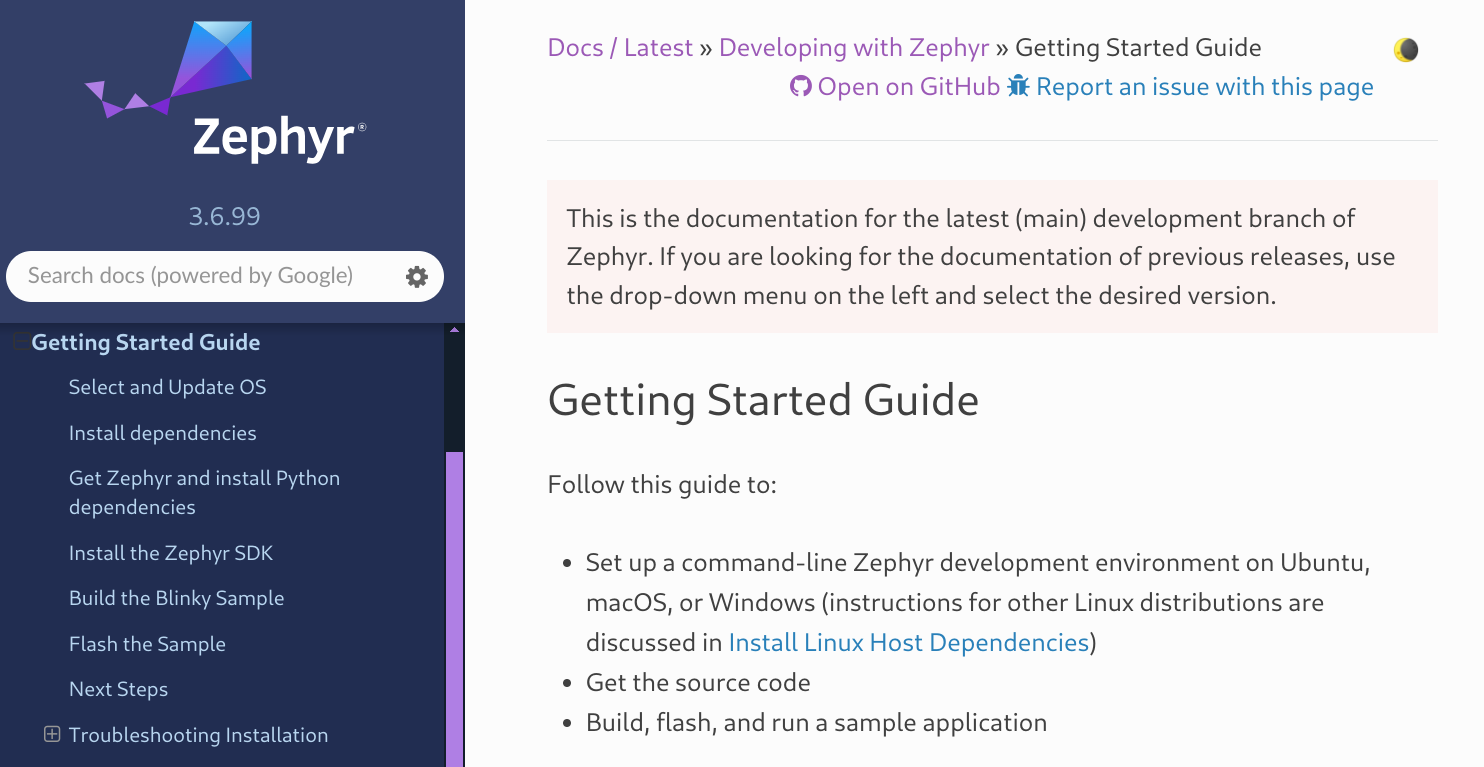
\includegraphics[width=0.9\textwidth]{images/zephyr_getting_started.png}
    \caption*{\scriptsize\href{https://docs.zephyrproject.org/latest/getting_started/index.html}{https://docs.zephyrproject.org/latest/getting\_started/index.html}}
  \end{figure}
\end{frame}
%%%%%%%%%%%%%%%%%%%%%%%%%%%%%%%%%%%%%%%%%%%%%%%%%%%%%%%%%%%%%%%%%%%%%%%%%%%%%%%
\begin{frame}[fragile]{Setting up a Local Development Environment}
Linux, macOS and Windows are supported!

Components:
  \begin{description}
    \item [Packages] git, cmake, python ..
    \item [Zephyr SDK] Toolchains for different architectures (compiler assembler..)
    \item [Python Tools] west, Install via requirements.txt in virtualenv
    \item [IDE] Text editor, IDE (e.g. VSCode)
    \item [Repositories] Zephyr, modules via west
  \end{description}
\end{frame}
%%%%%%%%%%%%%%%%%%%%%%%%%%%%%%%%%%%%%%%%%%%%%%%%%%%%%%%%%%%%%%%%%%%%%%%%%%%%%%%
\begin{frame}[fragile]{Testing the Local Development Environment}
  \begin{columns}
    \begin{column}{0.6\textwidth}
%-----------------------------------------
    Build and flash the application with \texttt{west}
    \begin{minted}[
      linenos,
      numbersep=15pt,
      framesep=2mm,
      bgcolor=lightgray!20,
      baselinestretch=1.1,
      fontsize=\scriptsize,
      firstnumber=1,
      stepnumber=5,
    ]{shell}
cd ~/zephyrproject/zephyr
west build -b reel_boad samples/basic/blinky -p
west flash
    \end{minted}
    \begin{minted}[
      linenos,
      numbersep=15pt,
      framesep=2mm,
      bgcolor=lightgray!20,
      baselinestretch=1.1,
      fontsize=\scriptsize,
      firstnumber=1,
      stepnumber=5,
    ]{shell}
cd ~/zephyrproject/zephyr
west build -b native_sim samples/hello_world/ -p
west build -t run
->
*** Booting Zephyr OS build v3.6.0 ***
Hello World! native_sim
    \end{minted}
%-----------------------------------------
    \end{column}
    \begin{column}{0.4\textwidth}
      \begin{figure}
        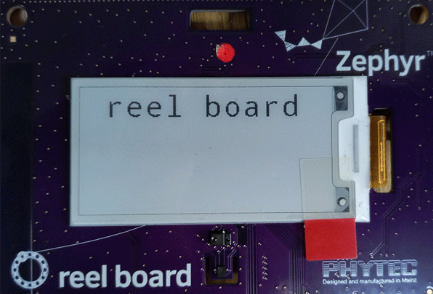
\includegraphics[width=0.8\textwidth]{images/zephyr_blinky.png}
        \caption*{reel board with blinking LED}
      \end{figure}
    \end{column}
  \end{columns}
\end{frame}
%%%%%%%%%%%%%%%%%%%%%%%%%%%%%%%%%%%%%%%%%%%%%%%%%%%%%%%%%%%%%%%%%%%%%%%%%%%%%%%
\begin{frame}[fragile]{Starting a Cloud Development Environment}
  \begin{columns}
    \begin{column}{0.6\textwidth}
%-----------------------------------------
    GitHub Codespaces \footnotemark
    \begin{itemize}
      \item Cloud hosted development environment based on devcontainers
      \item Visual Studio Code integration
      \item Runs on Microsoft Azure cloud
      \item Configuration individual for each repository
    \end{itemize}
%-----------------------------------------
    \end{column}
    \begin{column}{0.4\textwidth}
      \begin{figure}
        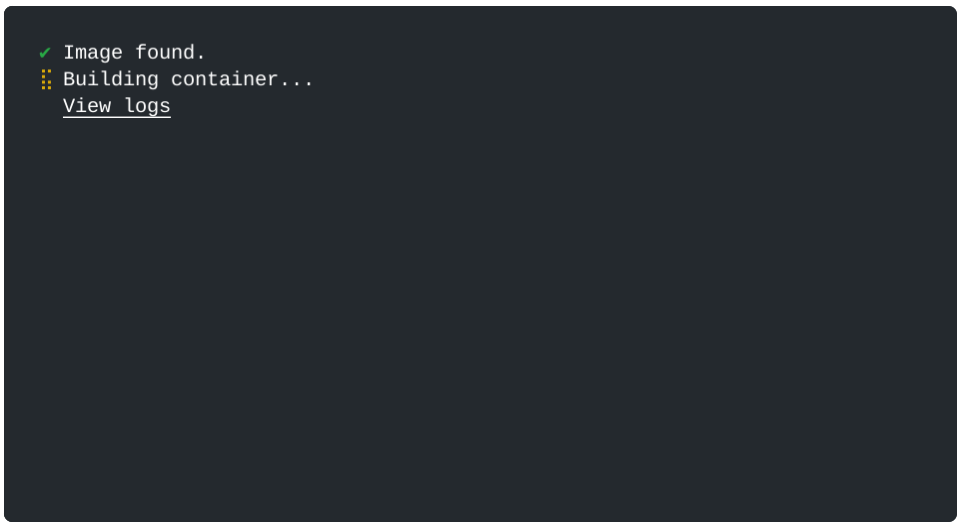
\includegraphics[width=1.1\textwidth]{images/codespaces_setting_up.png}
        \caption*{Codespaces starting..}
      \end{figure}
    \end{column}
  \end{columns}
  \footnotetext{Open Source Alternatives: Gitpod, Eclipse Theia and many more}
\end{frame}
%%%%%%%%%%%%%%%%%%%%%%%%%%%%%%%%%%%%%%%%%%%%%%%%%%%%%%%%%%%%%%%%%%%%%%%%%%%%%%%
\begin{frame}[fragile]{Active Instance of GitHub Codespace}
  \begin{columns}
    \begin{column}{0.4\textwidth}
      \begin{figure}
        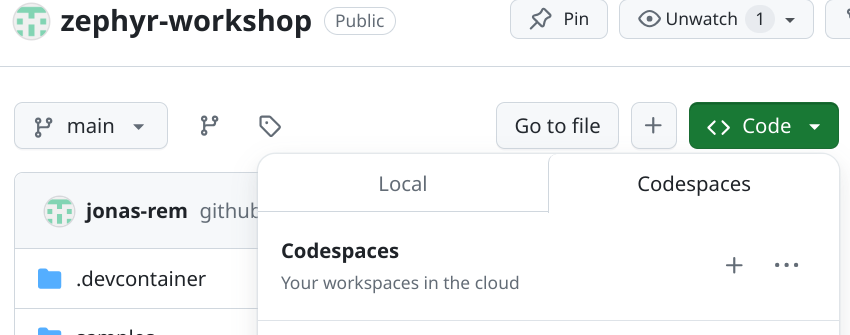
\includegraphics[width=\textwidth]{images/codespaces_how_to_start.png}
        \caption{Create a new Codespace}
      \end{figure}
      \begin{figure}
        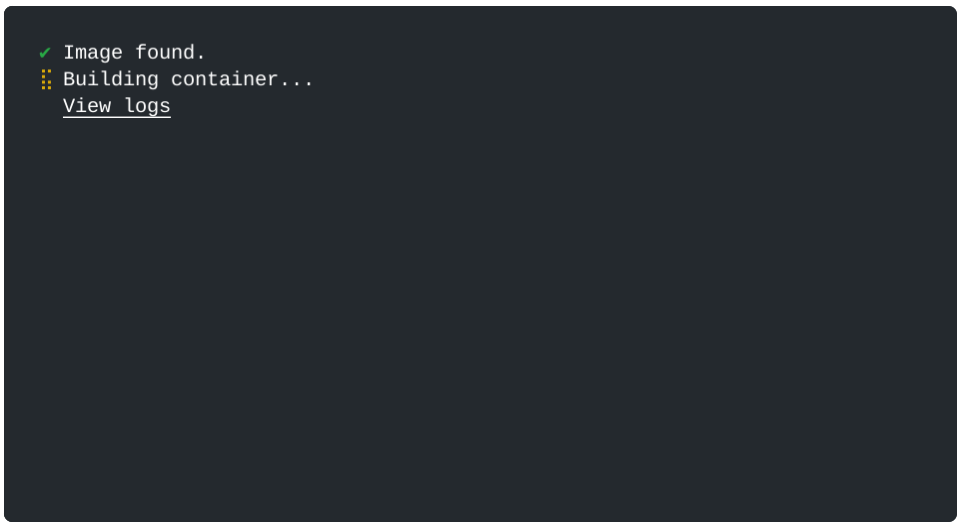
\includegraphics[width=0.7\textwidth]{images/codespaces_setting_up.png}
        \caption{Codespaces starting..}
      \end{figure}
    \end{column}
    \begin{column}{0.6\textwidth}
      \begin{figure}
        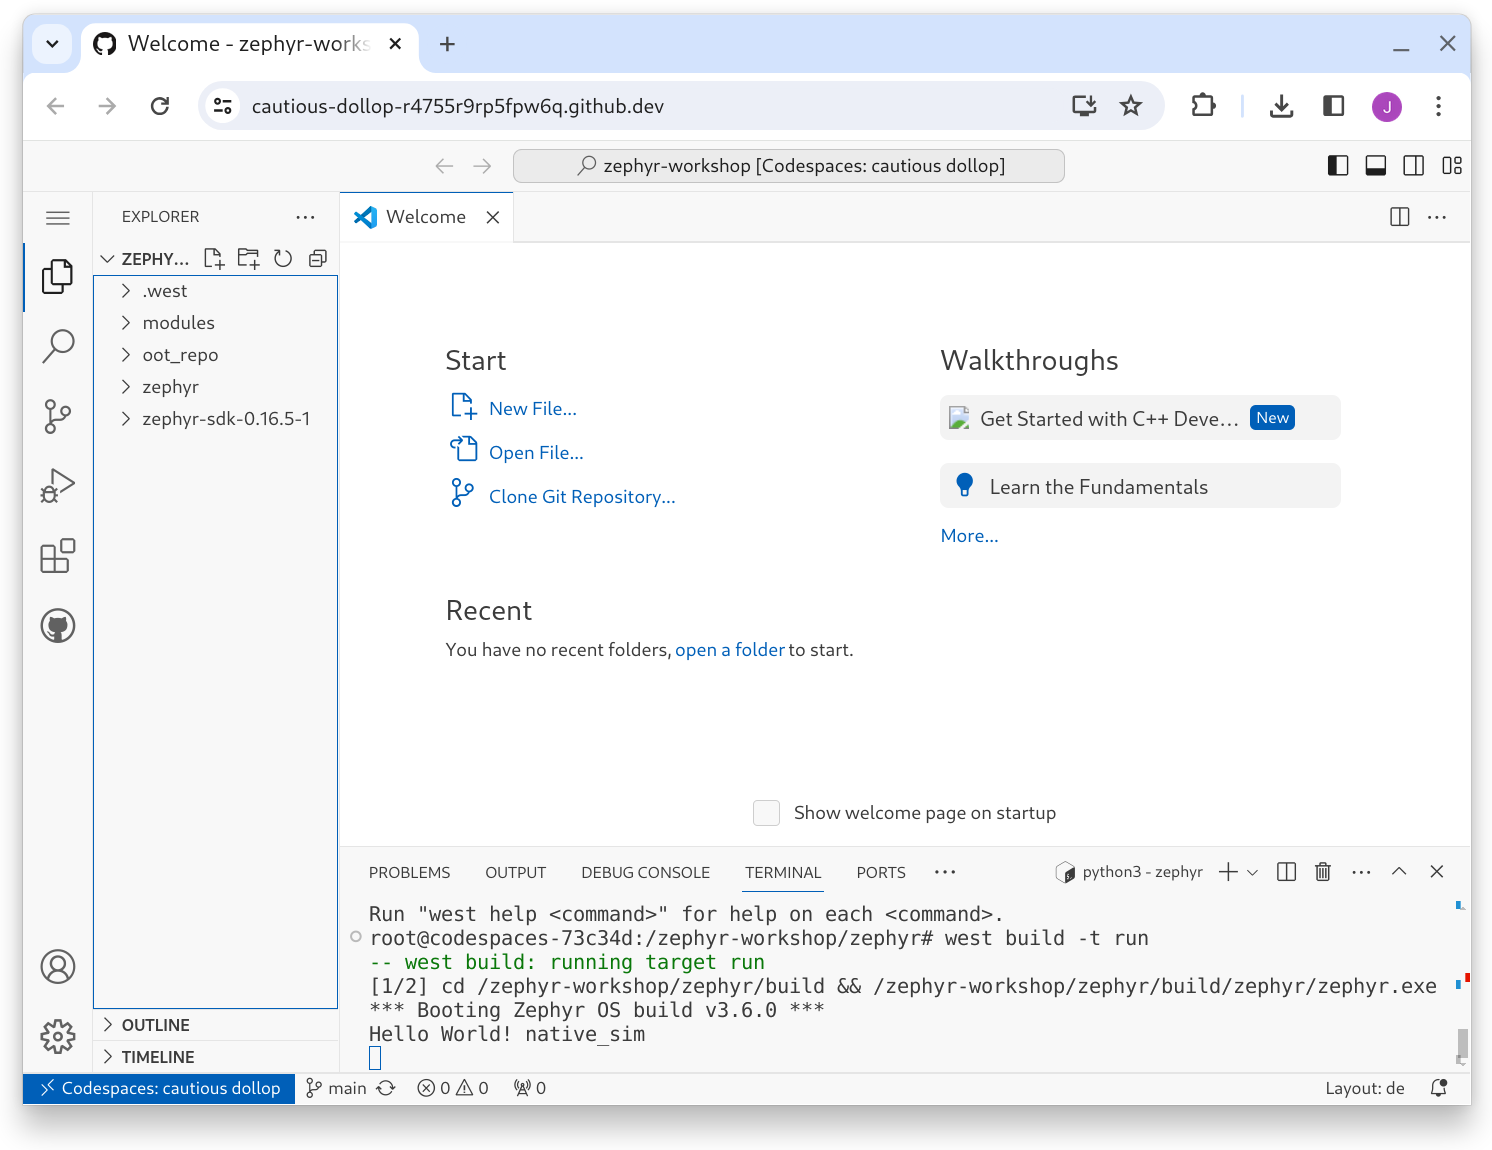
\includegraphics[width=\textwidth]{images/codespaces_open.png}
        \caption{Codespaces in a Browser Window}
      \end{figure}
    \end{column}
  \end{columns}
\end{frame}
%%%%%%%%%%%%%%%%%%%%%%%%%%%%%%%%%%%%%%%%%%%%%%%%%%%%%%%%%%%%%%%%%%%%%%%%%%%%%%%
\begin{frame}[fragile]{Recommendations from my Experience}
Virtual Machines in combination with hardware can bring their own problems.

Prioritize a local environment over a cloud environment
  \begin{itemize}
    \item Hardware is better accessible
    \item Better integration of your own tools
  \end{itemize}

        Check vendor tools that can enhance your Zephyr Dev Environment
\end{frame}
%%%%%%%%%%%%%%%%%%%%%%%%%%%%%%%%%%%%%%%%%%%%%%%%%%%%%%%%%%%%%%%%%%%%%%%%%%%%%%%
\subsection{Hands-on 1}
\begin{frame}[fragile]{But for Showcasing, Codespaces is great! - Hands-on 1}
  \begin{columns}
    \begin{column}{0.6\textwidth}
            Start your own Codespaces Instance now! \footnotemark[1] \footnotemark[2]

      \href{https://github.com/jonas-rem/zephyr-workshop}{github.com/jonas-rem/zephyr-workshop}

      Setup will take a few minutes..

      Test your setup with the Hello World example:
      \begin{itemize}
        \item \scriptsize west build -b native\_sim zephyr/samples/hello\_world -p
        \item \scriptsize west build -t run
      \end{itemize}
    \end{column}
    \begin{column}{0.4\textwidth}
      \begin{figure}
        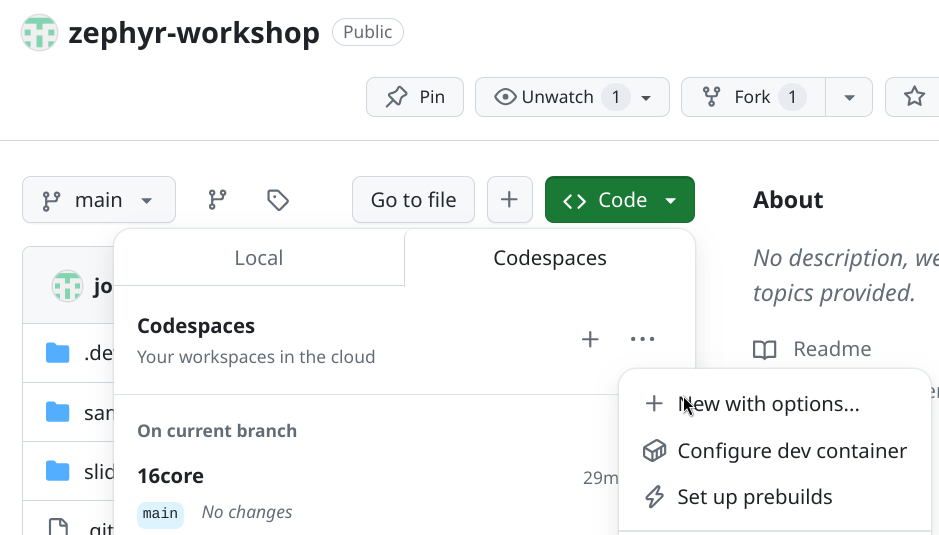
\includegraphics[width=1.1\textwidth]{images/codespaces_setting_up_class.png}
        \caption*{Setup new Instance}
      \end{figure}
    \end{column}
  \end{columns}
        \footnotetext[1]{\textbf{Recommendation:} Use a 4-core setup instead of
                         the 2-core default.}
        \footnotetext[2]{\textbf{Note:} You should have 120 core-hours per month free.}
\end{frame}
%%%%%%%%%%%%%%%%%%%%%%%%%%%%%%%%%%%%%%%%%%%%%%%%%%%%%%%%%%%%%%%%%%%%%%%%%%%%%%%
\section{Code Examples and Subsystems}
% Explain simple code examples
% Showcase the Codespaces environment to everyone
% Let the audience try out the Codespaces environment, give a coding task
% -> Timer and workqueue example
%%%%%%%%%%%%%%%%%%%%%%%%%%%%%%%%%%%%%%%%%%%%%%%%%%%%%%%%%%%%%%%%%%%%%%%%%%%%%%%
\begin{frame}[fragile]{Samples in Zephyr}

  \begin{block}{Samples}
    \begin{itemize}
      \item Zephyr provides a wide range of samples
      \item Samples are located in \texttt{zephyr/samples/}
      \item Isolated functionality or feature
    \end{itemize}
  \end{block}
  \begin{block}{Tests}
    \begin{itemize}
      \item Tests are located in \texttt{zephyr/tests/}
      \item Isolated test cases for a feature or hardware
      \item Useful to test e.g. a device driver
    \end{itemize}
  \end{block}
  \begin{block}{Applications}
    \begin{itemize}
      \item Application Example: {\scriptsize \url{https://github.com/zephyrproject-rtos/example-application}}
      \item ZSWatch - Open Source Smart Watch: {\scriptsize \url{https://github.com/jakkra/ZSWatch}}
    \end{itemize}
  \end{block}
\end{frame}
%%%%%%%%%%%%%%%%%%%%%%%%%%%%%%%%%%%%%%%%%%%%%%%%%%%%%%%%%%%%%%%%%%%%%%%%%%%%%%%
\begin{frame}[fragile]{01\_hello\_world}
  \begin{columns}
    \begin{column}{0.6\textwidth}
%-----------------------------------------
      \begin{description}
        \item [Description] Simple Hello World program \footnotemark
        \item [Learn] Test setup
        \item Structure of a Zephyr application
      \end{description}
      \begin{block}{Build and run}
      \begin{itemize}
        \item \scriptsize west build -b qemu\_cortex\_m0 samples/01\_hello\_world -p
        \item \scriptsize west build -t run
      \end{itemize}
      \end{block}
%-----------------------------------------
    \end{column}
    \begin{column}{0.4\textwidth}
        {\fontsize{7}{7}\selectfont
          \begin{verbatim}
samples/01_hello_world/
├── CMakeLists.txt
├── prj.conf
├── README.rst
├── sample.yaml
├── 01_hello_world
└── src
    └── main.c
          \end{verbatim}
        }
    \end{column}
  \end{columns}
  \footnotetext{Equivalent in the Zephyr main Repository: zephyr/samples/hello\_world.}
\end{frame}
%%%%%%%%%%%%%%%%%%%%%%%%%%%%%%%%%%%%%%%%%%%%%%%%%%%%%%%%%%%%%%%%%%%%%%%%%%%%%%%
\begin{frame}[fragile]{01\_hello\_world Configuring the Build System}
\inputmintedpath{cmake}{../samples/01_hello_world/CMakeLists.txt}
\end{frame}
%%%%%%%%%%%%%%%%%%%%%%%%%%%%%%%%%%%%%%%%%%%%%%%%%%%%%%%%%%%%%%%%%%%%%%%%%%%%%%%
\begin{frame}[fragile]{01\_hello\_world Application Source Code}
\inputmintedpath{c}{../samples/01_hello_world/src/main.c}
\end{frame}
%%%%%%%%%%%%%%%%%%%%%%%%%%%%%%%%%%%%%%%%%%%%%%%%%%%%%%%%%%%%%%%%%%%%%%%%%%%%%%
\begin{frame}[fragile]{01\_hello\_world Application Build Output}
  \begin{listing}[H]
    \begin{minted}[
      linenos,
      numbersep=15pt,
      framesep=2mm,
      bgcolor=lightgray!20,
      baselinestretch=1.1,
      fontsize=\scriptsize,
      firstnumber=1,
      stepnumber=5,
    ]{shell}
west build -b qemu_cortex_m0 samples/01_hello_world/ -p
-- Found host-tools: zephyr 0.16.5 (/home/jonas/Downloads/zephyr-sdk-0.16.5-1)
-- Found toolchain: zephyr 0.16.5 (/home/jonas/Downloads/zephyr-sdk-0.16.5-1)
[..]
Parsing /home/jonas/git/zephyrproject/zephyr/Kconfig
-- The C compiler identification is GNU 12.2.0
-- The CXX compiler identification is GNU 12.2.0
-- The ASM compiler identification is GNU
-- Using ccache: /usr/bin/ccache
-- Configuring done (2.5s)
-- Generating done (0.0s)
-- Build files have been written to: /home/jonas/git/zephyrproject/zephyr-workshop/build
-- west build: building application
[1/123] Preparing syscall dependency handling

[2/123] Generating include/generated/version.h
-- Zephyr version: 3.6.0 (/home/jonas/git/zephyrproject/zephyr), build: v3.6.0
[122/123] Linking C executable zephyr/zephyr.elf
Memory region         Used Size  Region Size  %age Used
           FLASH:       14414 B       256 KB      5.50%
             RAM:        3928 B        16 KB     23.97%
        IDT_LIST:          0 GB        32 KB      0.00%
    \end{minted}
  \caption{\scriptsize{Console Output}}
  \end{listing}
\end{frame}
%%%%%%%%%%%%%%%%%%%%%%%%%%%%%%%%%%%%%%%%%%%%%%%%%%%%%%%%%%%%%%%%%%%%%%%%%%%%%%%
\begin{frame}[fragile]{01\_hello\_world Build Artifacts}
  \begin{columns}
    \begin{column}{0.6\textwidth}
%-----------------------------------------
      \begin{description}
        \item [Build Location] \texttt{build/}
        \item [Executable Location] \texttt{build/zephyr/}
        \item [Artifacts]
          \begin{itemize}
            \item \texttt{zephyr.elf|hex|bin}
            \item \texttt{zephyr.map}
            \item \texttt{autoconf.h} (Kconfig options)
            \item \texttt{libapp.a} (Application library)
            \item \texttt{Kconfig.dts} (Device tree conf)
          \end{itemize}
      \end{description}
%-----------------------------------------
    \end{column}
    \begin{column}{0.4\textwidth}
        {\fontsize{7}{7}\selectfont
          \begin{verbatim}
build/
├── app
│   └── libapp.a
├── Kconfig
│   └── Kconfig.dts
└── zephyr
    ├── include
    │   └── generated
    │      ├── autoconf.h
    ├── zephyr.dts
    ├── zephyr.elf|bin|hex
    ├── zephyr_final.map
          \end{verbatim}
        }
    \end{column}
  \end{columns}
\end{frame}
%%%%%%%%%%%%%%%%%%%%%%%%%%%%%%%%%%%%%%%%%%%%%%%%%%%%%%%%%%%%%%%%%%%%%%%%%%%%%%%
\begin{frame}[fragile]{01\_hello\_world Sample - Console Output}
  \begin{listing}[H]
    \begin{minted}[
      linenos,
      numbersep=15pt,
      framesep=2mm,
      bgcolor=lightgray!20,
      baselinestretch=1.1,
      fontsize=\scriptsize,
      firstnumber=1,
      stepnumber=5,
    ]{shell}
*** Booting Zephyr OS build v3.6.0-214-gf1011b3c8265 ***
Hello World! qemu_cortex_m0
    \end{minted}
  \caption{\scriptsize{Console Output}}
  \end{listing}
\end{frame}
%%%%%%%%%%%%%%%%%%%%%%%%%%%%%%%%%%%%%%%%%%%%%%%%%%%%%%%%%%%%%%%%%%%%%%%%%%%%%%%
\begin{frame}[fragile]{02\_logging Sample}
  \begin{columns}
    \begin{column}{0.6\textwidth}
      \begin{description}
	\item [Description] Logging subsystem example\footnotemark
	\item [Logging] Log levels
	\item Set loglevel via Kconfig
	\item Different Logging backends, e.g. filesystem, BLE
	\item Log messages printed in own thread when system is idle
	\item [Sample] Demonstrates logging output
      \end{description}
    \end{column}
    \begin{column}{0.4\textwidth}
        {\fontsize{6}{6}\selectfont
  \begin{listing}[H]
    \begin{minted}[
      framesep=2mm,
      bgcolor=lightgray!20,
      baselinestretch=1.1,
      fontsize=\tiny,
    ]{Kconfig}
CONFIG_LOG=y
    \end{minted}
    \caption{\scriptsize{Excerpt from samples/02\_logging/prj.conf}}
  \end{listing}
  \begin{listing}[H]
    \begin{minted}[
      framesep=2mm,
      bgcolor=lightgray!20,
      baselinestretch=1.1,
      fontsize=\tiny,
    ]{c}
#include <zephyr/logging/log.h>

LOG_MODULE_REGISTER(hello_world, LOG_LEVEL_DBG);

int main(void)
{
	LOG_INF("info string");

	return 0;
}
    \end{minted}
  \caption{\scriptsize{Excerpt from samples/02\_logging/src/main.c}}
  \end{listing}
        }
    \end{column}
  \end{columns}
  \footnotetext{Equivalent in the Zephyr main Repository: zephyr/samples/subsys/logging/logger.}
\end{frame}
%%%%%%%%%%%%%%%%%%%%%%%%%%%%%%%%%%%%%%%%%%%%%%%%%%%%%%%%%%%%%%%%%%%%%%%%%%%%%%%
\begin{frame}[fragile]{02\_logging Sample - Console Output}
  \begin{listing}[H]
    \begin{minted}[
      linenos,
      numbersep=15pt,
      framesep=2mm,
      bgcolor=lightgray!20,
      baselinestretch=1.1,
      fontsize=\scriptsize,
      firstnumber=1,
      stepnumber=5,
    ]{shell}
*** Booting Zephyr OS build v3.6.0-1981-g1f55be8b42df ***
Hello World! qemu_cortex_m0
[00:00:00.002,446] <err> hello_world: error string
[00:00:00.002,653] <dbg> hello_world: main: debug string
[00:00:00.002,675] <inf> hello_world: info string
[00:00:00.002,698] <dbg> hello_world: main: int8_t 1, uint8_t 2
[00:00:00.002,718] <dbg> hello_world: main: int16_t 16, uint16_t 17
[00:00:00.002,736] <dbg> hello_world: main: int32_t 32, uint32_t 33
[00:00:00.002,758] <dbg> hello_world: main: int64_t 64, uint64_t 65
[00:00:00.002,814] <dbg> hello_world: main: char !
[00:00:00.003,164] <dbg> hello_world: main: s str static str c str
[00:00:00.003,346] <dbg> hello_world: main: d str dynamic str
[00:00:00.003,399] <dbg> hello_world: main: mixed str dynamic str --- dynamic str --- _ --- _
[00:00:00.003,440] <dbg> hello_world: main: mixed c/s ! static str dynamic str static str !
[00:00:00.003,458] <dbg> hello_world: main: pointer 0x5b1a
[00:00:00.003,489] <dbg> hello_world: main: HeXdUmP!
                        48 45 58 44 55 4d 50 21  20 23 40                |HEXDUMP!  #@     

    \end{minted}
  \end{listing}
\end{frame}
%%%%%%%%%%%%%%%%%%%%%%%%%%%%%%%%%%%%%%%%%%%%%%%%%%%%%%%%%%%%%%%%%%%%%%%%%%%%%%%
\begin{frame}[fragile]{03\_workqueues Sample}
      \begin{description}
	\item [Description] Workqueue and Timer Example
	\item [Learn] Workqueue, Timers, Runtime Contexts (IRQ, Thread)
	\item Queue of work items
	\item Work items are executed in a thread context
	\item Timer is used to schedule work items
	\item System workqueue is enabled by default
	\item [Sample] Executes a function in different contexts
      \end{description}
\end{frame}
%%%%%%%%%%%%%%%%%%%%%%%%%%%%%%%%%%%%%%%%%%%%%%%%%%%%%%%%%%%%%%%%%%%%%%%%%%%%%%%
\begin{frame}[fragile]{03\_workqueues Sample - Console Output}
  \begin{listing}[H]
    \begin{minted}[
      linenos,
      numbersep=15pt,
      framesep=2mm,
      bgcolor=lightgray!20,
      baselinestretch=1.1,
      fontsize=\scriptsize,
      firstnumber=1,
      stepnumber=5,
    ]{shell}
*** Booting Zephyr OS build v3.6.0-1981-g1f55be8b42df ***
Work Item Executed - runtime context:
 Thread Name: main 
 Thread Priority: 0 

Work Item Executed - runtime context:
 Thread Name: sysworkq 
 Thread Priority: -1 

Work Item Executed - runtime context:
 Thread Name: my_work_q_thread 
 Thread Priority: 5 

Timer Expired!!
Work Item Executed - runtime context:
 ISR Context!

Work Item Executed - runtime context:
 Thread Name: sysworkq 
 Thread Priority: -1
    \end{minted}
  \end{listing}
\end{frame}
%%%%%%%%%%%%%%%%%%%%%%%%%%%%%%%%%%%%%%%%%%%%%%%%%%%%%%%%%%%%%%%%%%%%%%%%%%%%%%%
\begin{frame}[fragile]{04\_shell Sample}
  \begin{columns}
    \begin{column}{0.6\textwidth}
      \begin{description}
	\item [Description] Shell subsystem example\footnotemark
	\item [Shell] Command line interface
	\item Command history, completion, help
	\item Great for testing and debugging
	\item [Sample] Provides a basic shell
      \end{description}
    \end{column}
    \begin{column}{0.4\textwidth}
        {\fontsize{6}{6}\selectfont
  \begin{listing}[H]
    \begin{minted}[
      framesep=2mm,
      bgcolor=lightgray!20,
      baselinestretch=1.1,
      fontsize=\tiny,
    ]{Kconfig}
CONFIG_SHELL=y

# Optional features
CONFIG_THREAD_STACK_INFO=y
CONFIG_KERNEL_SHELL=y
CONFIG_THREAD_MONITOR=y
CONFIG_BOOT_BANNER=n
CONFIG_THREAD_NAME=y
CONFIG_DEVICE_SHELL=y
CONFIG_POSIX_CLOCK=y
CONFIG_DATE_SHELL=y
CONFIG_THREAD_RUNTIME_STATS=y
CONFIG_THREAD_RUNTIME_STATS_USE_TIMING_FUNCTIONS=y
CONFIG_STATS=y
CONFIG_STATS_SHELL=y
    \end{minted}
    \caption{\scriptsize{Excerpt from samples/04\_shell/prj.conf}}
  \end{listing}
        }
    \end{column}
  \end{columns}
  \footnotetext{Equivalent in the Zephyr main Repository: zephyr/samples/subsys/shell/shell\_module.}
\end{frame}
%%%%%%%%%%%%%%%%%%%%%%%%%%%%%%%%%%%%%%%%%%%%%%%%%%%%%%%%%%%%%%%%%%%%%%%%%%%%%%%
\begin{frame}[fragile]{04\_shell Sample - Console Output}
  \begin{listing}[H]
    \begin{minted}[
      linenos,
      numbersep=15pt,
      framesep=2mm,
      bgcolor=lightgray!20,
      baselinestretch=1.1,
      fontsize=\tiny,
      firstnumber=1,
      stepnumber=5,
    ]{shell}
uart:~$
  bypass              clear               date
  demo                device              devmem
  dynamic             help                history
  kernel              log_test            rem
uart:~$ kernel threads
Threads:
 0x20000c70 sysworkq
	options: 0x0, priority: -1 timeout: 0
	state: pending, entry: 0x7315
	Total execution cycles: 207 (0 %)
	stack size 1024, unused 808, usage 216 / 1024 (21 %)

*0x200006d0 shell_uart
	options: 0x0, priority: 14 timeout: 0
	state: queued, entry: 0x3c8d
	Total execution cycles: 19143 (0 %)
	stack size 2048, unused 924, usage 1124 / 2048 (54 %)

 0x200001c8 logging
	options: 0x0, priority: 14 timeout: 0
	state: pending, entry: 0x19d1
	Total execution cycles: 289 (0 %)
	stack size 768, unused 576, usage 192 / 768 (25 %)

 0x20000a80 idle
	options: 0x1, priority: 15 timeout: 0
	state: , entry: 0xad31
	Total execution cycles: 7795318 (99 %)
	stack size 256, unused 168, usage 88 / 256 (34 %)
    \end{minted}
  \end{listing}
\end{frame}
%%%%%%%%%%%%%%%%%%%%%%%%%%%%%%%%%%%%%%%%%%%%%%%%%%%%%%%%%%%%%%%%%%%%%%%%%%%%%%%
\begin{frame}[fragile]{05\_sensor Sample}
  \begin{columns}
    \begin{column}{0.6\textwidth}
      \begin{description}
	\item [Description] TI HDC1010: I2C Temperature and Humidity Sensor
	\item [Sensor] Temperature and Humidity e.g. on the reel board
	\item [Sample] Demonstrates Sensor API
      \end{description}
    \end{column}
    \begin{column}{0.4\textwidth}
        {\fontsize{5}{5}\selectfont
  \begin{listing}[H]
    \begin{minted}[
      framesep=2mm,
      bgcolor=lightgray!20,
      baselinestretch=1.1,
      fontsize=\tiny,
    ]{c}
sensor_sample_fetch(dev);
sensor_channel_get(dev, SENSOR_CHAN_AMBIENT_TEMP,
	           &temp);
sensor_channel_get(dev, SENSOR_CHAN_HUMIDITY,
	           &humidity);

/* print the result */
printk("Temp = %d.%06d C, RH = %d.%06d %%\n",
       temp.val1, temp.val2,
       humidity.val1, humidity.val2);
    \end{minted}
    \caption{\scriptsize{Excerpt from samples/05\_sensor/src/main.c}}
  \end{listing}
        }
    \end{column}
  \end{columns}
  \footnotetext{Equivalent in the Zephyr main Repository: zephyr/samples/sensor/ti\_hdc.}
\end{frame}
%%%%%%%%%%%%%%%%%%%%%%%%%%%%%%%%%%%%%%%%%%%%%%%%%%%%%%%%%%%%%%%%%%%%%%%%%%%%%%%
\begin{frame}[fragile]{05\_sensor Sample - Console Output}
  \begin{listing}[H]
    \begin{minted}[
      linenos,
      numbersep=15pt,
      framesep=2mm,
      bgcolor=lightgray!20,
      baselinestretch=1.1,
      fontsize=\tiny,
      firstnumber=1,
      stepnumber=5,
    ]{shell}
*** Booting Zephyr OS build v3.6.0-1981-g1f55be8b42df ***
Dev 0x8090 name ti_hdc@43 is ready!
Fetching...
Temp = 23.778381 C, RH = 51.892089 %
Fetching...
Temp = 23.869018 C, RH = 51.470947 %
Fetching...
    \end{minted}
  \end{listing}
\end{frame}
%%%%%%%%%%%%%%%%%%%%%%%%%%%%%%%%%%%%%%%%%%%%%%%%%%%%%%%%%%%%%%%%%%%%%%%%%%%%%%%
\begin{frame}[fragile]{06\_ble Sample}
  \begin{columns}
    \begin{column}{0.6\textwidth}
      \begin{description}
     \item
	\item [Description] BLE Peripheral device, temperature monitor
	\item [Sample] App to connect: nRF Connect for Mobile (Android, iOS)
      \end{description}
    \end{column}
    \begin{column}{0.4\textwidth}
        {\fontsize{6}{6}\selectfont
  \begin{listing}[H]
    \begin{minted}[
      framesep=2mm,
      bgcolor=lightgray!20,
      baselinestretch=1.1,
      fontsize=\tiny,
    ]{Kconfig}
CONFIG_BT=y
CONFIG_LOG=y
CONFIG_BT_SMP=y
CONFIG_BT_PERIPHERAL=y
CONFIG_BT_DIS=y
CONFIG_BT_DIS_PNP=n
CONFIG_BT_BAS=y
CONFIG_BT_DEVICE_NAME="Zephyr Health Thermometer"
CONFIG_BT_DEVICE_APPEARANCE=768
CONFIG_CBPRINTF_FP_SUPPORT=y
    \end{minted}
    \caption{\scriptsize{Excerpt from samples/06\_ble/prj.conf}}
  \end{listing}
        }
    \end{column}
  \end{columns}
  \footnotetext{Equivalent in the Zephyr main Repository: zephyr/samples/bluetooth/peripheral\_ht.}
\end{frame}
%%%%%%%%%%%%%%%%%%%%%%%%%%%%%%%%%%%%%%%%%%%%%%%%%%%%%%%%%%%%%%%%%%%%%%%%%%%%%%%
\begin{frame}[fragile]{06\_ble Sample - Console Output}
  \begin{listing}[H]
    \begin{minted}[
      linenos,
      numbersep=15pt,
      framesep=2mm,
      bgcolor=lightgray!20,
      baselinestretch=1.1,
      fontsize=\tiny,
      firstnumber=1,
      stepnumber=5,
    ]{shell}
*** Booting Zephyr OS build v3.6.0-1981-g1f55be8b42df ***
[00:00:00.375,701] <inf> bt_hci_core: HW Platform: Nordic Semiconductor (0x0002)
[00:00:00.375,732] <inf> bt_hci_core: HW Variant: nRF52x (0x0002)
[00:00:00.375,762] <inf> bt_hci_core: Firmware: Standard Bluetooth controller (0x00) Version 3.6 Build 99
[00:00:00.376,495] <inf> bt_hci_core: Identity: CC:42:FB:73:2F:36 (random)
[00:00:00.376,525] <inf> bt_hci_core: HCI: version 5.4 (0x0d) revision 0x0000, manufacturer 0x05f1
[00:00:00.376,556] <inf> bt_hci_core: LMP: version 5.4 (0x0d) subver 0xffff
Bluetooth initialized
temp device is 0x26824, name is temp@4000c000
Advertising successfully started
Connected
temperature is 24C
temperature is 23.75C
Indication success
Indication complete
Indication success
Indication complete
temperature is 23.75C
temperature is 24C
    \end{minted}
  \end{listing}
\end{frame}
%%%%%%%%%%%%%%%%%%%%%%%%%%%%%%%%%%%%%%%%%%%%%%%%%%%%%%%%%%%%%%%%%%%%%%%%%%%%%%%
\begin{frame}[fragile]{06\_ble Sample - Connect with a Smartphone}
  \begin{columns}
    \begin{column}{0.5\textwidth}
      \begin{figure}
        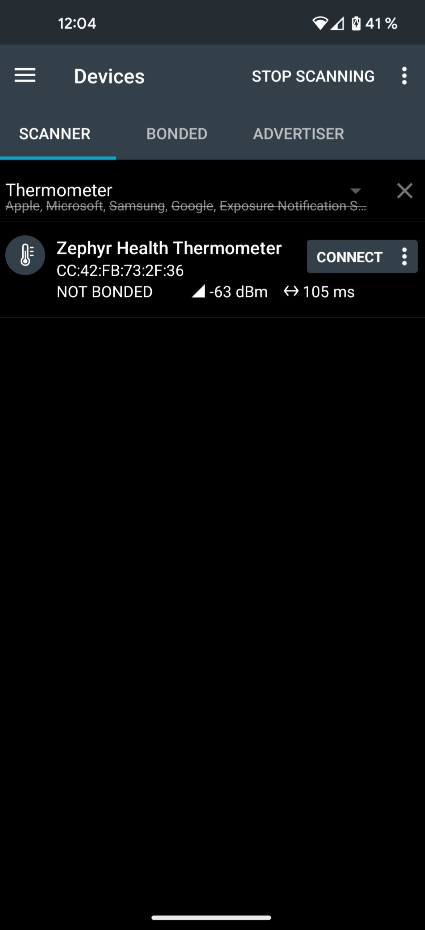
\includegraphics[width=0.4\textwidth]{images/nrf_connect_scan.png}
        \caption*{Scanning for BLE devices}
      \end{figure}
    \end{column}
    \begin{column}{0.5\textwidth}
      \begin{figure}
        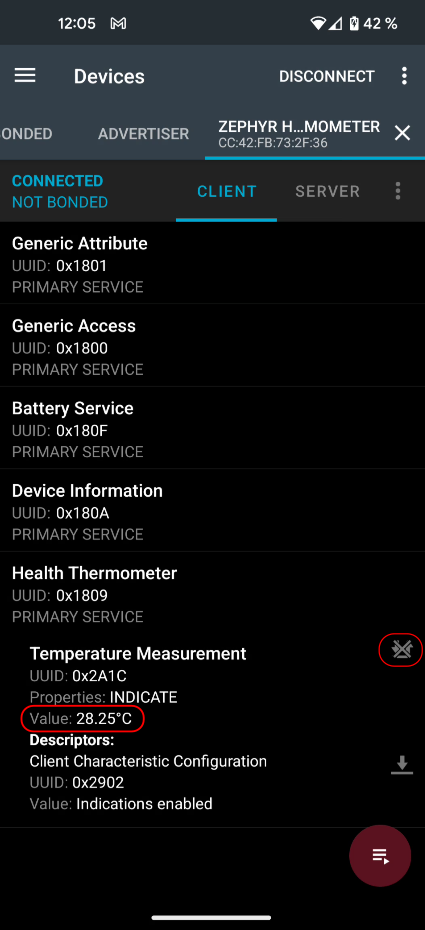
\includegraphics[width=0.4\textwidth]{images/nrf_connect_ble_connected.png}
        \caption*{Connected with nRF Connect App}
      \end{figure}
    \end{column}
  \end{columns}
\end{frame}
%%%%%%%%%%%%%%%%%%%%%%%%%%%%%%%%%%%%%%%%%%%%%%%%%%%%%%%%%%%%%%%%%%%%%%%%%%%%%%%
\subsection{Hands-on 2}
\begin{frame}[fragile]{Test the Samples - Hands-on 2}
  \begin{columns}
    \begin{column}{0.6\textwidth}
     Navigate to the zephyr-workshop repository.
      \begin{itemize}
        \item \scriptsize cd zephyr-workshop
      \end{itemize}

      Build and run the samples\footnotemark[1]:
      \begin{itemize}
        \item \scriptsize west build -b qemu\_cortex\_m0 samples/02\_logging -p
        \item \scriptsize west build -t run
      \end{itemize}
    \end{column}
    \begin{column}{0.4\textwidth}
        {\fontsize{7}{7}\selectfont
          \begin{verbatim}
samples
├── 01_hello_world
├── 02_logging
├── 03_workqueues
├── 04_shell
├── 05_sensor
└── 06_ble
        \end{verbatim}
      }
    \end{column}
  \end{columns}
  \footnotetext[1]{\textbf{Note:} The sensor and ble samples require a
  board to run, you can skip them for now.}
\end{frame}
%%%%%%%%%%%%%%%%%%%%%%%%%%%%%%%%%%%%%%%%%%%%%%%%%%%%%%%%%%%%%%%%%%%%%%%%%%%%%%%
\section{Workspace Application and Hardware Abstraction}
% Out of Tree Build
% Explain devicetree
% Conditional Compilation (Different Code for different Boards)
% Coding Session 2 - Test on multiple boards
%%%%%%%%%%%%%%%%%%%%%%%%%%%%%%%%%%%%%%%%%%%%%%%%%%%%%%%%%%%%%%%%%%%%%%%%%%%%%%%
\begin{frame}[fragile]{Workspace Application}
  \begin{columns}
    \begin{column}{0.6\textwidth}
%-----------------------------------------
      \textbf{Workspace application} or \textbf{Out of tree} build \footnotemark[1]

      Separate application from Zephyr repository
      \begin{itemize}
        \item Independent version control for app
        \item Different Licences for app?
        \item Maintain references to Zephyr, Modules.. in app repo
        \item Update Zephyr version independently from app
      \end{itemize}

      Examples at \footnotemark[2] \footnotemark[3]
%-----------------------------------------
    \end{column}
    \begin{column}{0.4\textwidth}
        {\fontsize{7}{7}\selectfont
          \begin{verbatim}
zephyrproject
├── modules
│   └── hal
├── zephyr
│   ├── samples
│   ├── west.yml
└── zephyr-workshop (app)
    ├── west.yml
    └── samples
        └── 01_hello_world
            ├── CMakeLists.txt
            ├── prj.conf
            ├── README.rst
            ├── sample.yaml
            └── src
       \end{verbatim}
        }
    \end{column}
  \end{columns}
        \footnotetext[1]{\tiny\url{https://docs.zephyrproject.org/latest/develop/application/index.html}}
        \footnotetext[2]{\tiny\url{https://github.com/zephyrproject-rtos/example-application}}
        \footnotetext[2]{\tiny\url{https://github.com/jonas-rem/zephyr-workshop}}
\end{frame}
%%%%%%%%%%%%%%%%%%%%%%%%%%%%%%%%%%%%%%%%%%%%%%%%%%%%%%%%%%%%%%%%%%%%%%%%%%%%%%%
\begin{frame}[fragile]{Enabled by \texttt{west} and Manifest files}
  Manifests references repositories and modules \footnotemark[1]

  \begin{listing}[H]
    \begin{minted}[
      linenos,
      numbersep=15pt,
      framesep=2mm,
      bgcolor=lightgray!20,
      baselinestretch=1.1,
      fontsize=\scriptsize,
      firstnumber=1,
      stepnumber=5,
    ]{yaml}
manifest:
  remotes:
    - name: zephyrproject-rtos
      url-base: https://github.com/zephyrproject-rtos

  projects:
    - name: zephyr
      remote: zephyrproject-rtos
      revision: v3.6.0
      import:
        name-allowlist:
          - cmsis
          - hal_nordic
          - hal_nxp
          - [..]
    \end{minted}
    \caption{\scriptsize{\texttt{west.yaml} Manifest file in the zephyr-workshop repository}}
  \end{listing}
  \footnotetext[1]{\tiny\url{https://docs.zephyrproject.org/latest/develop/west/manifest.html}}
\end{frame}
%%%%%%%%%%%%%%%%%%%%%%%%%%%%%%%%%%%%%%%%%%%%%%%%%%%%%%%%%%%%%%%%%%%%%%%%%%%%%%%
\begin{frame}[fragile]{Understanding and Using \texttt{west}}
  \begin{columns}
    \begin{column}{0.6\textwidth}
      \texttt{west} repository management tool, developed by the Zephyr community
      \begin{itemize}
        \item Inspired by Google's Repo tool and git submodules
        \item Cloning Zephyr repo, dependencies, modules
        \item Keeping project repositories synchronized
        \item In addition building, flashing, and debugging support
      \end{itemize}

    \end{column}
    \begin{column}{0.4\textwidth}
        {\fontsize{6}{6}\selectfont
  \begin{listing}[H]
    \begin{minted}[
      framesep=2mm,
      bgcolor=lightgray!20,
      baselinestretch=1.1,
      fontsize=\tiny,
    ]{shell}
# Navigate to the project root
$ cd zephyrproject

# Update all repositories
$ west update

=== updating zephyr (zephyr):
HEAD is now at 468eb56cf24 [..]
=== updating cmsis (modules/hal/cmsis):
HEAD is now at 4b96cbb [..]
=== updating hal_atmel (modules/hal/atmel):
HEAD is now at aad79bf [..]
    \end{minted}
  \end{listing}
        }
    \end{column}
  \end{columns}
\end{frame}
%%%%%%%%%%%%%%%%%%%%%%%%%%%%%%%%%%%%%%%%%%%%%%%%%%%%%%%%%%%%%%%%%%%%%%%%%%%%%%%
\begin{frame}[fragile]{Application Structure - Use Case I}
  \begin{columns}
    \begin{column}{0.6\textwidth}
      \begin{description}
         \item[Who] User creates one application for testing
         \item[What] One variant of an application
         \item[Solution] Make changes inside the Zephyr tree for simplicity \footnotemark
      \end{description}
    \end{column}
    \begin{column}{0.4\textwidth}
      \begin{figure}
        \hspace*{1.5cm}
        \includesvg[width=0.8\textwidth]{images/application_topologies_1.svg}
      \end{figure}
    \end{column}
  \end{columns}
  \footnotetext{Not recommended production, use an out-of-tree build instead. This makes it easier to upgrade to more recent Zephyr versions.}
\end{frame}
%%%%%%%%%%%%%%%%%%%%%%%%%%%%%%%%%%%%%%%%%%%%%%%%%%%%%%%%%%%%%%%%%%%%%%%%%%%%%%%
\begin{frame}[fragile]{Application Structure - Use Case II}
  \begin{columns}
    \begin{column}{0.6\textwidth}
      \begin{description}
         \item[Who] One company developing one product
         \item [What] Two variants of the product
         \item Different sensors, pin assignments, but similar application
         \item[Solution] Devicetrees for each variant
         \item board\_a.dts: {\scriptsize\texttt{west build -b board\_a app}}
         \item board\_b.dts: {\scriptsize\texttt{west build -b board\_b app}}
      \end{description}
    \end{column}
    \begin{column}{0.4\textwidth}
      \begin{figure}
        \hspace*{0.4cm}
        \includesvg[width=\textwidth]{images/application_topologies_2.svg}
      \end{figure}
    \end{column}
  \end{columns}
\end{frame}
%%%%%%%%%%%%%%%%%%%%%%%%%%%%%%%%%%%%%%%%%%%%%%%%%%%%%%%%%%%%%%%%%%%%%%%%%%%%%%%
\begin{frame}[fragile]{Application Structure - Use Case III}
  \begin{columns}
    \begin{column}{0.6\textwidth}
      \begin{description}
         \item[Who] One company developing multiple products
         \item[What] Different applications
         \item[Solution] Seperate applications
         \item Use same Zephyr version for all applications if you can
      \end{description}
    \end{column}
    \begin{column}{0.4\textwidth}
      \begin{figure}
        \hspace*{-0.5cm}
        \includesvg[width=1.17\textwidth]{images/application_topologies_3.svg}
      \end{figure}
    \end{column}
  \end{columns}
\end{frame}
%%%%%%%%%%%%%%%%%%%%%%%%%%%%%%%%%%%%%%%%%%%%%%%%%%%%%%%%%%%%%%%%%%%%%%%%%%%%%%%
\begin{frame}[fragile]{Application Structure - Use Case IV}
  \begin{columns}
    \begin{column}{0.6\textwidth}
      \begin{description}
         \item[Who] Service provider developing different products for multiple companies
         \item[What] Development states and lifecycle for products differ
         \item[Solution] Individual manifest files for each product
         \item Create your own modules, share code inbetween projects
         \item Quickly setup and reference projecs with west
      \end{description}
    \end{column}
    \begin{column}{0.4\textwidth}
      \begin{figure}
        \hspace*{-0.5cm}
        \includesvg[width=1.17\textwidth]{images/application_topologies_4.svg}
      \end{figure}
    \end{column}
  \end{columns}
\end{frame}
%%%%%%%%%%%%%%%%%%%%%%%%%%%%%%%%%%%%%%%%%%%%%%%%%%%%%%%%%%%%%%%%%%%%%%%%%%%%%%%
\begin{frame}[fragile]{Zephyr Hardware Abstraction}
  \begin{columns}
    \begin{column}{0.6\textwidth}
%-----------------------------------------
      \begin{description}
          \item [Vendor HALs] Hardware abstraction available from vendors.
                  Abstracted via Zephyr APIs and drivers
          \item [Devicetree] Decouples the application from the hardware
          \item [Architecture] ARM, RISC-V, x86, ARC, NIOS II, Tensilica, Xtensa
          \item [Other] 600+ boards, 180+ sensors
      \end{description}
%-----------------------------------------
    \end{column}
    \begin{column}{0.4\textwidth}
      \begin{listing}[H]
        \begin{minted}[
          framesep=2mm,
          bgcolor=lightgray!20,
          baselinestretch=1.1,
          fontsize=\tiny,
        ]{console}
zephyrproject/zephyr:~$ ls arch/
arc    CMakeLists.txt  mips   riscv  xtensa
arm    common          nios2  sparc
arm64  Kconfig         posix  x86

zephyrproject:~$ ls modules/hal/
altera        espressif   nordic      silabs
ambiq         ethos_u     nuvoton     st
atmel         gigadevice  nxp         stm32
cirrus-logic  infineon    openisa     telink
[..]

zephyrproject/zephyr:~$ ls boards/
96boards               firefly       qemu
actinius               gd            rak
adafruit               google        raspberrypi
digilent               nordic        u-blox
enjoydigital           phytec        wemos
espressif              pine64        wiznet
[..]

zephyrproject/zephyr:~$ ls drivers/sensor/
adxl367                max30101
hs300x                 sht4x
ina3221                tcs3400
isl29035               th02
lps22hb                vl53l1x
[..]
        \end{minted}
      \end{listing}
    \end{column}
  \end{columns}
\end{frame}
%%%%%%%%%%%%%%%%%%%%%%%%%%%%%%%%%%%%%%%%%%%%%%%%%%%%%%%%%%%%%%%%%%%%%%%%%%%%%%%
\begin{frame}[fragile]{Zephyr Hardware Abstraction - devicetree}
  \begin{columns}
    \begin{column}{0.6\textwidth}
      Describes the available hardware
        \begin{itemize}
          \item Proven concept used in the Linux kernel
          \item Single source for hardware information
          \item Drivers and source are hardware independent
        \end{itemize}

      In Zephyr: C header generation at compile time
    \end{column}
    \begin{column}{0.4\textwidth}
      \begin{figure}
        \hspace*{-0.5cm}
        \includesvg[width=0.6\textwidth]{images/devicetree-logo.svg}
              \caption*{devicetree Logo\footnotemark}
      \end{figure}
      \footnotetext{\tiny\url{https://www.devicetree.org/}}
    \end{column}
  \end{columns}
\end{frame}
%%%%%%%%%%%%%%%%%%%%%%%%%%%%%%%%%%%%%%%%%%%%%%%%%%%%%%%%%%%%%%%%%%%%%%%%%%%%%%%
\begin{frame}[fragile]{Zephyr Hardware Abstraction - devicetree}
  \begin{listing}[H]
    \begin{minted}[
      framesep=2mm,
      bgcolor=lightgray!20,
      baselinestretch=1.1,
      fontsize=\tiny,
    ]{dts}
arduino_i2c: &i2c0 {
        compatible = "nordic,nrf-twim";
        status = "okay";
        clock-frequency = <I2C_BITRATE_FAST>;

        pinctrl-0 = <&i2c0_default>;
        pinctrl-1 = <&i2c0_sleep>;
        pinctrl-names = "default", "sleep";
        mma8642fc: mma8652fc@1d {
                compatible = "nxp,fxos8700","nxp,mma8652fc";
                reg = <0x1d>;
                int1-gpios = <&gpio0 24 GPIO_ACTIVE_LOW>;
                int2-gpios = <&gpio0 25 GPIO_ACTIVE_LOW>;
        };

        ti_hdc@43 {
                compatible = "ti,hdc","ti,hdc1010";
                reg = <0x43>;
                drdy-gpios = <&gpio0 22 (GPIO_ACTIVE_LOW | GPIO_PULL_UP)>;
        };

        apds9960@39 {
                compatible = "avago,apds9960";
                reg = <0x39>;
                int-gpios = <&gpio0 23 (GPIO_ACTIVE_LOW | GPIO_PULL_UP)>;
        };
};
    \end{minted}
          \caption{\scriptsize{devicetree node for the reel board: \texttt{boards/phytec/reel\_board/dts/reel\_board.dtsi}}}
  \end{listing}
\end{frame}
%%%%%%%%%%%%%%%%%%%%%%%%%%%%%%%%%%%%%%%%%%%%%%%%%%%%%%%%%%%%%%%%%%%%%%%%%%%%%%%
\subsection{Hands-on 3}
\begin{frame}[fragile]{Let's build Zephyr for multiple boards! - Hands-on 3}
  \begin{columns}
    \begin{column}{0.6\textwidth}
       Take a random board. Find out if it is supported (Zephyr Docs).

       Build the blinky sample for your board:
       \begin{itemize}
               \item \scriptsize\texttt{west build -b <board> zephyr/samples/basic/blinky -p}
       \end{itemize}

       Flash\footnotemark[1] and check if the led is blinking:
       \begin{itemize}
         \item \scriptsize\texttt{west flash}
       \end{itemize}

    \end{column}
    \begin{column}{0.4\textwidth}
      \begin{figure}
        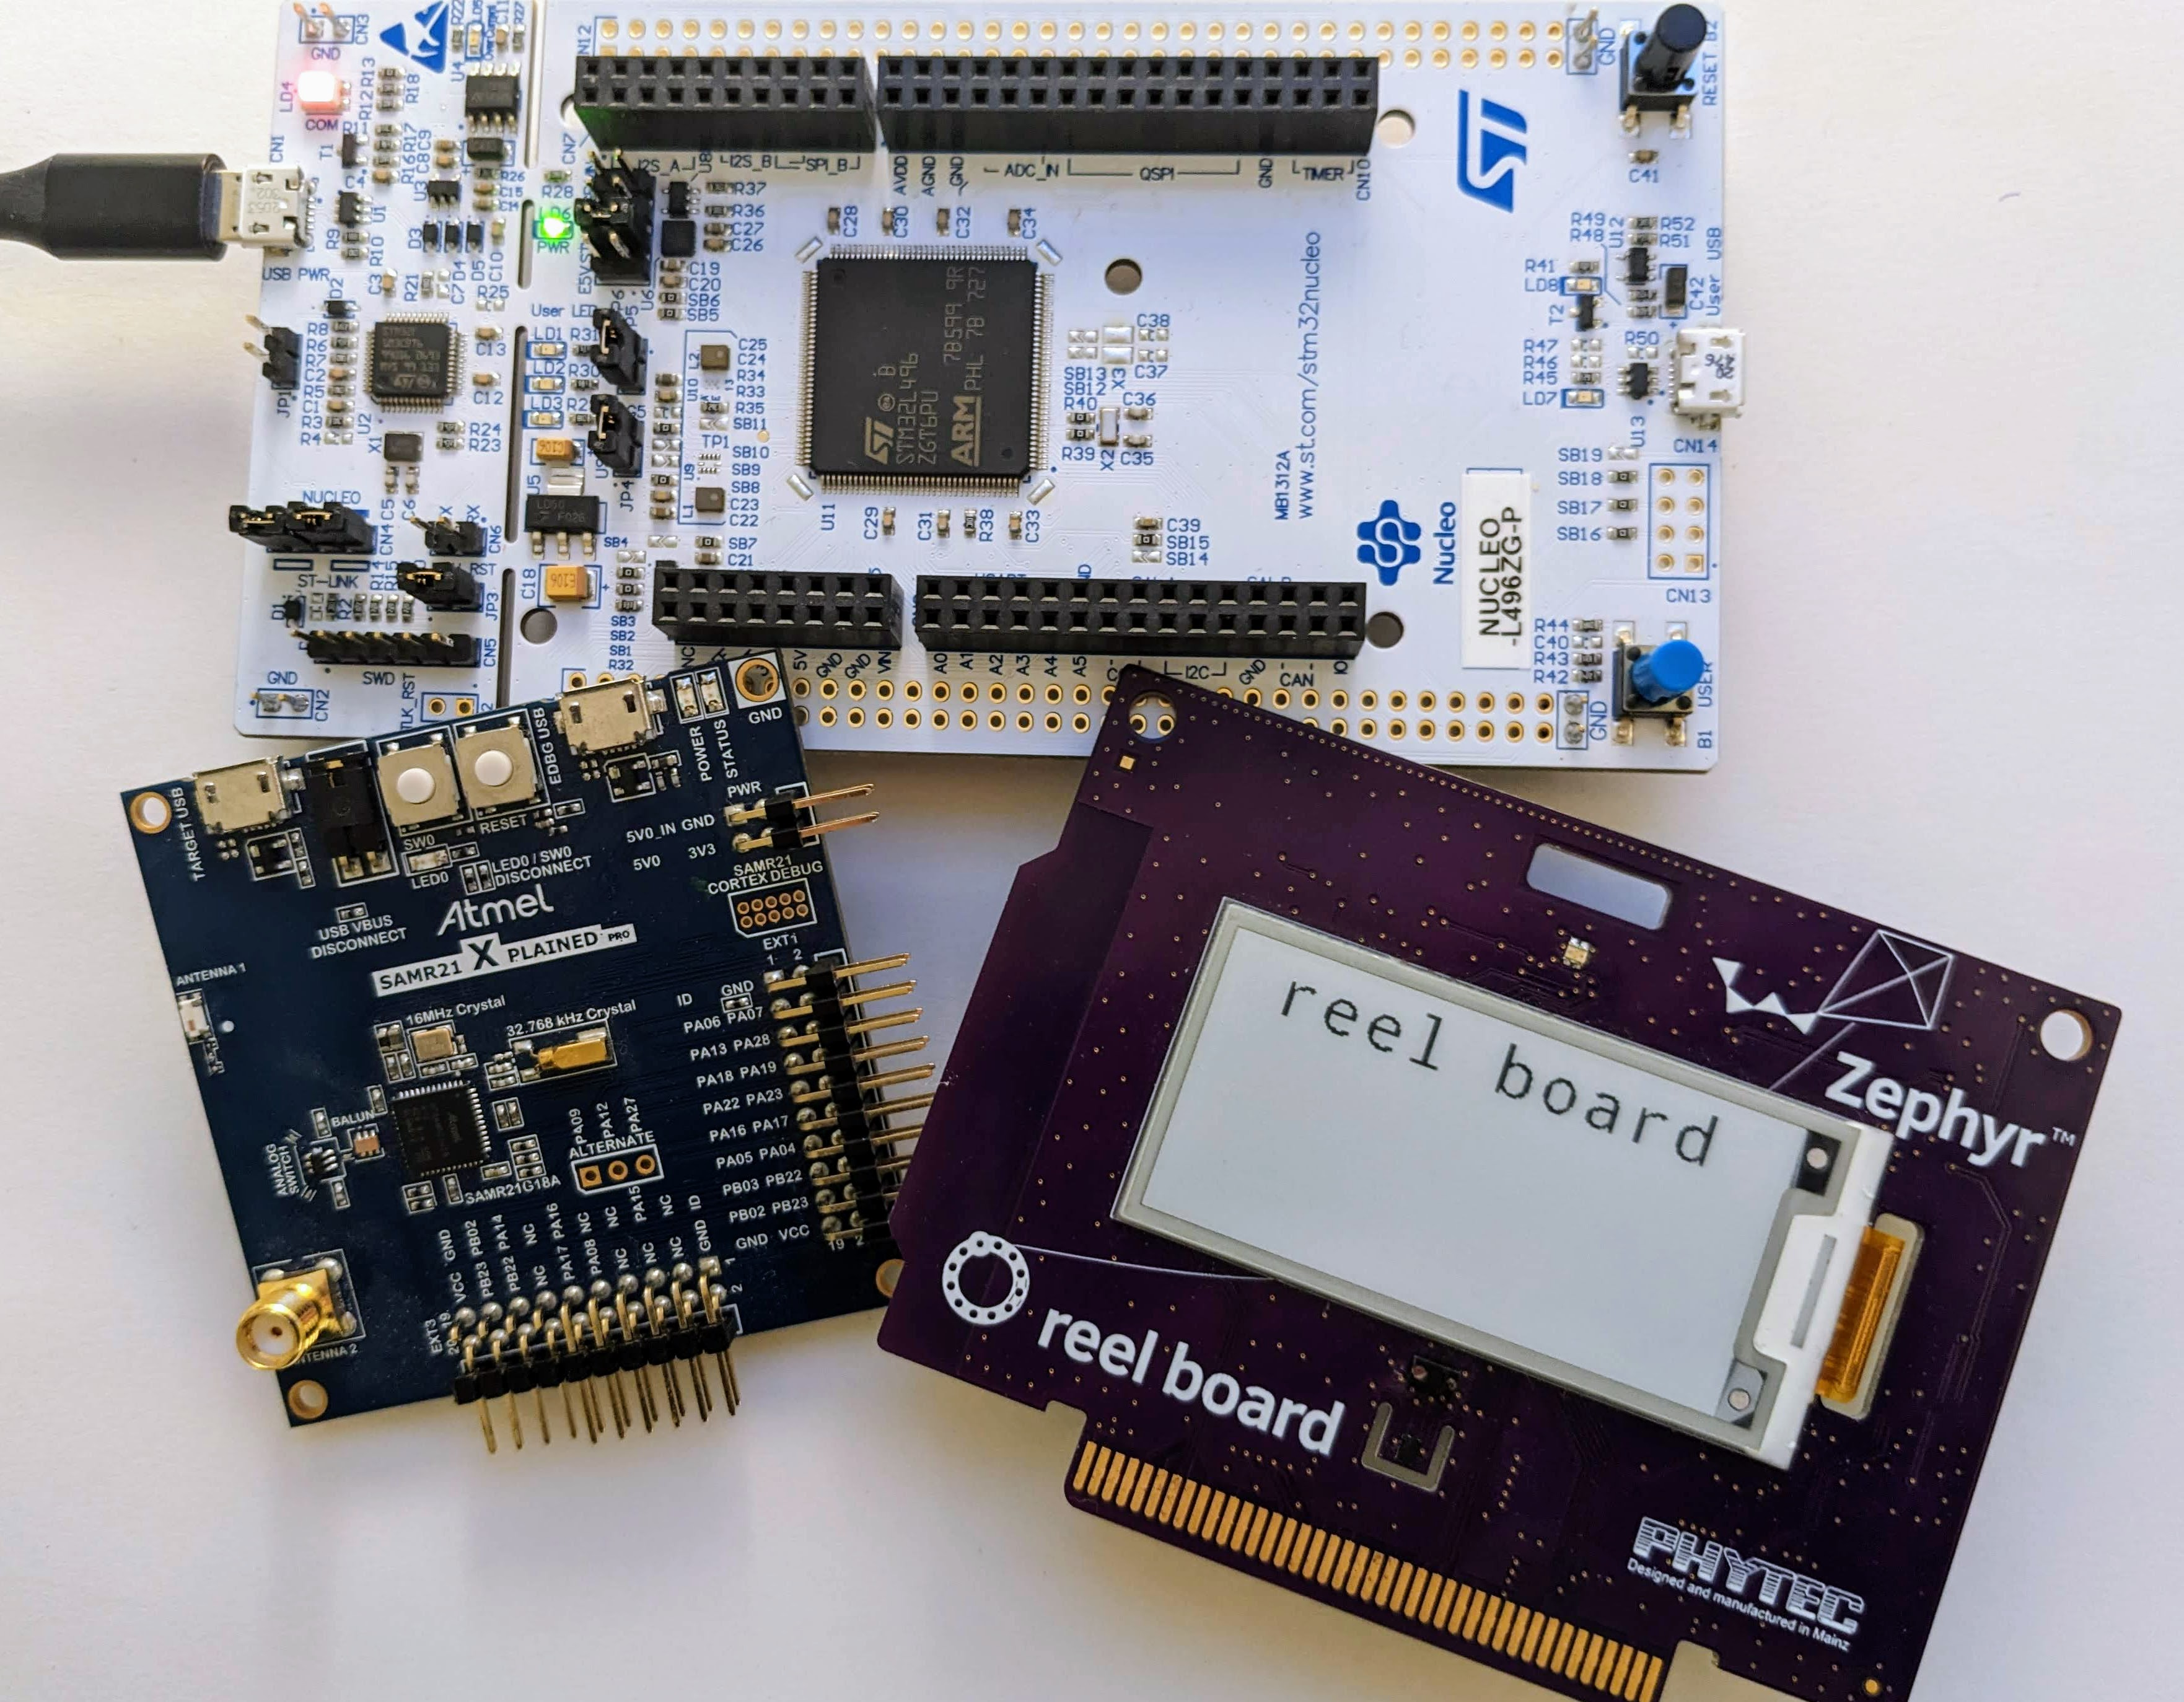
\includegraphics[width=1.1\textwidth]{images/boards.jpg}
        \caption*{Boards from different vendors}
      \end{figure}
    \end{column}
  \end{columns}
        \footnotetext[1]{Flashing is not supported from Codespaces. Download
        \texttt{build/zephyr/zephyr.hex}, send the file to j.remmert@phytec.de
        or copy to a USB stick and I will flash it for you.}
\end{frame}
%%%%%%%%%%%%%%%%%%%%%%%%%%%%%%%%%%%%%%%%%%%%%%%%%%%%%%%%%%%%%%%%%%%%%%%%%%%%%%%
\section{Application Development}
% zbus, IPC, Threads
% Work with modularization, utlize the build system
% Hands On Excersies 4 - Extend a sample application
%%%%%%%%%%%%%%%%%%%%%%%%%%%%%%%%%%%%%%%%%%%%%%%%%%%%%%%%%%%%%%%%%%%%%%%%%%%%%%%
\begin{frame}[fragile]{IPC Mechanisms and Zephyr bus (Zbus)}
  \begin{columns}
    \begin{column}{0.6\textwidth}
%-----------------------------------------
      Mutexes, Semaphores

      Conditional Variables, Message Queues

      Polling API to wait for any out of multiple conditions

    \begin{block}{Zbus}
      \begin{itemize}
        \item Comparable to D-Bus in Linux
        \item Many-to-many communication
        \item Simplifies thread synchronization
      \end{itemize}
    \end{block}
%-----------------------------------------
    \end{column}
    \begin{column}{0.4\textwidth}
      \begin{figure}
       \includesvg[width=\textwidth]{images/zbus_zephyr.svg}
        \caption*{Zbus overview\footnotemark}
      \end{figure}
    \end{column}
  \end{columns}
  \footnotetext{\tiny\url{https://docs.zephyrproject.org/latest/services/zbus/index.html}}
\end{frame}
%%%%%%%%%%%%%%%%%%%%%%%%%%%%%%%%%%%%%%%%%%%%%%%%%%%%%%%%%%%%%%%%%%%%%%%%%%%%%%%
\begin{frame}[fragile]{Example Application}
  \begin{columns}
    \begin{column}{0.6\textwidth}
%-----------------------------------------
    Button
    \begin{itemize}
      \item Switch between system states (active, sleep)
    \end{itemize}

    LED
    \begin{itemize}
      \item Indicate system state
      \item Run in own thread for smooth animations
    \end{itemize}
%-----------------------------------------
    \end{column}
    \begin{column}{0.4\textwidth}
      \begin{figure}
       \includesvg[width=0.9\textwidth]{images/zbus_application.svg}
        \caption*{Minimal modular application with zbus}
      \end{figure}
    \end{column}
  \end{columns}
\end{frame}
%%%%%%%%%%%%%%%%%%%%%%%%%%%%%%%%%%%%%%%%%%%%%%%%%%%%%%%%%%%%%%%%%%%%%%%%%%%%%%%
\begin{frame}[fragile]{Example Application - Modular Development}
  \begin{columns}
    \begin{column}{0.6\textwidth}
%-----------------------------------------
      \begin{description}
        \item [General] Code reuse, maintainability, readability
	\item [IPC] Communication e.g. via Zbus
	\item Context of each module can be controlled
	\item [Testing] Modules can be tested seperately
      \end{description}
%-----------------------------------------
    \end{column}
    \begin{column}{0.4\textwidth}
        {\fontsize{6}{6}\selectfont
          \begin{verbatim}
app/
├── CMakeLists.txt
├── Kconfig
├── prj.conf
└── src
    ├── common
    │   ├── CMakeLists.txt
    │   ├── message_channel.c
    │   └── message_channel.h
    ├── main.c
    └── modules
        ├── button
        │   ├── button.c
        │   ├── CMakeLists.txt
        │   └── Kconfig.button
        └── led
            ├── CMakeLists.txt
            ├── Kconfig.led
            └── led.c
          \end{verbatim}
        }
    \end{column}
  \end{columns}
\end{frame}
%%%%%%%%%%%%%%%%%%%%%%%%%%%%%%%%%%%%%%%%%%%%%%%%%%%%%%%%%%%%%%%%%%%%%%%%%%%%%%%
\begin{frame}[fragile]{Example Application - Testing}
  \begin{columns}
    \begin{column}{0.6\textwidth}
%-----------------------------------------
      Isolated testing of modules

      Add subsystems like shell, ztest for test cases

      Tests reference modules via CMake

      Interfaces inbetween modules abstracted via zbus
%-----------------------------------------
    \end{column}
    \begin{column}{0.4\textwidth}
        {\fontsize{6}{6}\selectfont
          \begin{verbatim}
test/
├── button
│   ├── CMakeLists.txt
│   ├── Kconfig
│   ├── prj.conf
│   ├── sample.yaml
│   └── src
│       └── main.c
└── led
    ├── CMakeLists.txt
    ├── Kconfig
    ├── prj.conf
    ├── sample.yaml
    └── src
        └── main.c
          \end{verbatim}
        }
    \end{column}
  \end{columns}
\end{frame}
%%%%%%%%%%%%%%%%%%%%%%%%%%%%%%%%%%%%%%%%%%%%%%%%%%%%%%%%%%%%%%%%%%%%%%%%%%%%%%%
\begin{frame}[fragile]{Example Application - Testing Modules}
  \begin{listing}[H]
    \begin{minted}[
      framesep=2mm,
      bgcolor=lightgray!20,
      baselinestretch=1.1,
      fontsize=\tiny,
    ]{cmake}
target_sources(app PRIVATE src/main.c)
add_subdirectory(../../app/src/common common)
add_subdirectory(../../app/src/modules/button button)
    \end{minted}
    \caption{\footnotesize{Excerpt from : \texttt{test/button/CMakeLists.txt}}}
  \end{listing}
  \begin{listing}[H]
    \begin{minted}[
      framesep=2mm,
      bgcolor=lightgray!20,
      baselinestretch=1.1,
      fontsize=\tiny,
    ]{c}
void button_test_msg_cb(const struct zbus_channel *chan)
{
	const enum sys_msg *msg_type;

	msg_type = zbus_chan_const_msg(chan);
	if (msg_type == SYS_BUTTON_PRESSED) {
		LOG_INF("Button pressed!");
	}
}

ZBUS_LISTENER_DEFINE(button_test, button_test_msg_cb);
ZBUS_CHAN_ADD_OBS(button_ch, button_test, DEFAULT_OBS_PRIO);
    \end{minted}
    \caption{\footnotesize{Excerpt from : \texttt{test/button/src/main.c}}}
  \end{listing}
\end{frame}
%%%%%%%%%%%%%%%%%%%%%%%%%%%%%%%%%%%%%%%%%%%%%%%%%%%%%%%%%%%%%%%%%%%%%%%%%%%%%%%
\begin{frame}[fragile]{Example Application - Automated Testing}
  \begin{columns}
    \begin{column}{0.6\textwidth}
%-----------------------------------------
      Zephyr Test Framework (Ztest)
      \begin{description}
        \item [twister] Test runner for Zephyr
        \item [Harness] ztest, test, console, pytest, gtest,robot
      \end{description}

      In this example, the integration test feature is used
      \begin{itemize}
          \item \scriptsize\texttt{west twister -T app/ -T test/ --integration}
      \end{itemize}
%-----------------------------------------
    \end{column}
    \begin{column}{0.4\textwidth}
        {\fontsize{7}{7}\selectfont
          \begin{verbatim}
app/sample.yaml
test/led/sample.yaml
test/button/sample.yaml
          \end{verbatim}
  \begin{listing}[H]
    \begin{minted}[
      framesep=2mm,
      bgcolor=lightgray!20,
      baselinestretch=1.1,
      fontsize=\tiny,
    ]{yaml}
integration_platforms:
  - reel_board
  - frdm_k64f
  - nucleo_wb55rg
  - nucleo_l496zg
  - mimxrt1010_evk
  - nucleo_l452re
  - nrf5340dk/nrf5340/cpuapp
  - stm32f4_disco
    \end{minted}
    \caption{\footnotesize{Excerpt from : \texttt{app/sample.yaml}}}
  \end{listing}
        }
    \end{column}
  \end{columns}
\end{frame}
%%%%%%%%%%%%%%%%%%%%%%%%%%%%%%%%%%%%%%%%%%%%%%%%%%%%%%%%%%%%%%%%%%%%%%%%%%%%%%%
\begin{frame}[fragile]{Example Application - Automated Testing Results}
  \begin{listing}[H]
    \begin{minted}[
      framesep=2mm,
      bgcolor=lightgray!20,
      baselinestretch=1.1,
      fontsize=\tiny,
    ]{console}
$ west twister -T app/ -T test/ --integration
INFO - Zephyr version: v3.6.0-1949-g2302e5f76621
INFO - Writing JSON report /home/jonas/git/zephyrproject/zephyr-workshop/twister-out/testplan.json
INFO - JOBS: 16
INFO - Total complete:   24/  24  100%  skipped:    0, failed:    0, error:    0
INFO - 3 test scenarios (24 test instances) selected, 0 configurations skipped (0 by static filter, 0 at runtime).
INFO - 24 of 24 test configurations passed (100.00%), 0 failed, 0 errored, 0 skipped with 0 warnings in 66.80 seconds
INFO - In total 0 test cases were executed, 24 skipped on 8 out of total 706 platforms (1.13%)
INFO - 0 test configurations executed on platforms, 24 test configurations were only built.
INFO - Saving reports...
INFO - Writing JSON report /home/jonas/git/zephyrproject/zephyr-workshop/twister-out/twister.json
INFO - Writing xunit report /home/jonas/git/zephyrproject/zephyr-workshop/twister-out/twister.xml...
INFO - Writing xunit report /home/jonas/git/zephyrproject/zephyr-workshop/twister-out/twister_report.xml...
INFO - Run completed
    \end{minted}
    \caption{\footnotesize{Console output for twister integration tests. In this examples there are only build tests, but tests that run on the hardware are possible.}}
  \end{listing}
\end{frame}
%%%%%%%%%%%%%%%%%%%%%%%%%%%%%%%%%%%%%%%%%%%%%%%%%%%%%%%%%%%%%%%%%%%%%%%%%%%%%%%
% TODO:
% - Add renode support,
% - Prepare the applicaiton for 3 states
\subsection{Hands-on 4}
\begin{frame}[fragile]{Extend the Application - Hands-on 4}
  \begin{columns}
    \begin{column}{0.6\textwidth}
      Currently there are two system states: \textbf{standby}, \textbf{sleep}.
      Extend the application with a third state: \textbf{active}. Iterate
      through states via buttonpress:
      \textbf{standby}->\textbf{sleep}->\textbf{active}\footnotemark[1]
      \begin{description}
        \item [Sleep] LED off
        \item [Standby] LED blinking
        \item [Active] LED on
      \end{description}
	    Renode\footnotemark[2] offers a way to simulate the application e.g. on the stm32f4\_discovery board.
    \end{column}
    \begin{column}{0.4\textwidth}
      \begin{listing}[H]
        \begin{minted}[
          framesep=2mm,
          bgcolor=lightgray!20,
          baselinestretch=1.1,
          fontsize=\tiny,
        ]{console}
Build led test or app
# west build -b stm32f4_disco test/led -p
# west build -b stm32f4_disco app -p
Start Simulation with Renode with last build binary:
# renode util/stm32f4.resc --disable-gui --console

Siumlate Button Press via Shell:
(target)# my_app button button_press

Simulate Button Press via Renode (not used here)
(STM32F4_Disco)# sysbus.gpioPortA.UserButton Press
(STM32F4_Disco)# sysbus.gpioPortA.UserButton Release

ESC followed by CRTL+d to exit renode

Run the integration tests with twister
# west twister -T app/ -T test/ --integration
        \end{minted}
        \caption{\footnotesize{Commands for build and simulation}}
      \end{listing}
    \end{column}
  \end{columns}
  \footnotetext[1]{You can start with the LED module and the test firmware at \texttt{test\//led}.}
\footnotetext[2]{\texttt{Renode} is an Open Source simulation framework for embedded systems from Antmicro.}
\end{frame}
%%%%%%%%%%%%%%%%%%%%%%%%%%%%%%%%%%%%%%%%%%%%%%%%%%%%%%%%%%%%%%%%%%%%%%%%%%%%%%%
\section{Summary}
%%%%%%%%%%%%%%%%%%%%%%%%%%%%%%%%%%%%%%%%%%%%%%%%%%%%%%%%%%%%%%%%%%%%%%%%%%%%%%%
\begin{frame}[fragile]{Key Points from the Workshop\footnotemark}
  \begin{columns}
    \begin{column}{0.6\textwidth}
%-----------------------------------------
      \begin{description}
        \item [Ecosystem] Many components around an RTOS, e.g.~drivers, networking
        \item Modular and hardware independent by default!
        \item Many concepts from Linux makes it easier to get started
        \item [Structure] Ready-to-use structure for your application
        \item Systems get more complex, avoid developing from scratch
      \end{description}
%-----------------------------------------
    \end{column}
    \begin{column}{0.4\textwidth}
      \begin{description}
        \item [Open Source] Supply chain security
        \item No vendor lock-in
        \item Supported by large companies
        \item [Community] Active, questions and contributions welcomed
      \end{description}
    \end{column}
  \end{columns}
  \footnotetext{\tiny Slides and the workshop material are available at \url{https://github.com/jonas-rem/zephyr-workshop}}
\end{frame}
%%%%%%%%%%%%%%%%%%%%%%%%%%%%%%%%%%%%%%%%%%%%%%%%%%%%%%%%%%%%%%%%%%%%%%%%%%%%%%%
\begin{frame}{Q and A}
  \centering
  \LARGE Questions?

  \footnotetext{\footnotesize{\ccbysa\hspace{0.2cm}This presentation is licensed under CC BY-SA.}}
\end{frame}
%%%%%%%%%%%%%%%%%%%%%%%%%%%%%%%%%%%%%%%%%%%%%%%%%%%%%%%%%%%%%%%%%%%%%%%%%%%%%%%
\appendix
\section*{Backup Slides}
%%%%%%%%%%%%%%%%%%%%%%%%%%%%%%%%%%%%%%%%%%%%%%%%%%%%%%%%%%%%%%%%%%%%%%%%%%%%%%%
\begin{frame}[fragile]{Renode: Technical Overview}
  \begin{itemize}
    \item Testing of embedded systems in a reproducible virtual environment
    \item Simulation of unmodified binaries for target hardware
    \item Simulates entire SoCs, including CPUs, peripherals, and interconnects
    \item Enables complex network simulations, both wired and wireless
    \item Allows for interactive debugging, system state inspection, and automated testing
    \item Open Source, actively developed by Antmicro
  \end{itemize}
\end{frame}
%%%%%%%%%%%%%%%%%%%%%%%%%%%%%%%%%%%%%%%%%%%%%%%%%%%%%%%%%%%%%%%%%%%%%%%%%%%%%%%
\end{document}
